\subsection{Scaling and Performance Characterization}

We first characterize the overheads of HTBAC and the runtime system. HTBAC
enables concurrent execution of multiple protocol instances. With each new
protocol instance generated for an application, the HTBAC overhead grows to
match the additional requirement of generating and coordinating protocols.

In order to understand the contribution of the various events in HTBAC, termed
as HTBAC overhead, to the total time to completion (TTC) we construct the
following: $TTC = TTX + T_{O}$ where
 \(TTX\) measures the execution duration across all task, including file
 staging, MD kernel execution, and post-executables, and $T_{O}$ the total
overhead is given by the sum of the constituent overheads: $$T_{O} =
T_{O}\textsuperscript{HTBAC} + T_{O}\textsuperscript{EnTK} +
T_{O}\textsuperscript{RP}$$


% \(Time-to-run =
% T(overhead\textsubscript{HTBAC} +
% T(overhead\textsubscript{entk}) +
% T(overhead\textsubscript{rp}) + T(execution)\).

% We define \(T(execution)\) as \(TTX = TTC - T_q\) where \(TTC\) is
% time-to-completion and \(T_q\) is time spent queuing on the HPC machine.



% T(overhead\textsubscript{HTBAC} +
% T(overhead\textsubscript{entk}) +
% T(overhead\textsubscript{rp}) + T(execution)\).

% We define \(T(execution)\) as \(TTX = TTC - T_q\) where \(TTC\) is
% time-to-completion and \(T_q\) is time spent queuing on the HPC machine.


\subsubsection{Weak Scaling Experiments}

Here we show weak scalability for the TIES protocol by growing the number of
protocol instances while adhering to the required number of pipelines. By
design of each protocol, an increase in the number of instances simply means
an increase in the number of pipelines. The first weak scalability experiment
demonstrates the behavior of HTBAC, EnTK and RP using the multiple instances
of the TIES protocol. By design of weak scaling, the ratio between the number
of pipelines and cores are kept constant. As the number of cores (measure of
resource) changes by a factor of 2, we introduce twice as many protocol
instances. As designed, the weak scaling property provides insight into the
size of the workload that can be investigated in a given amount of time.

\begin{figure}
  \centering
   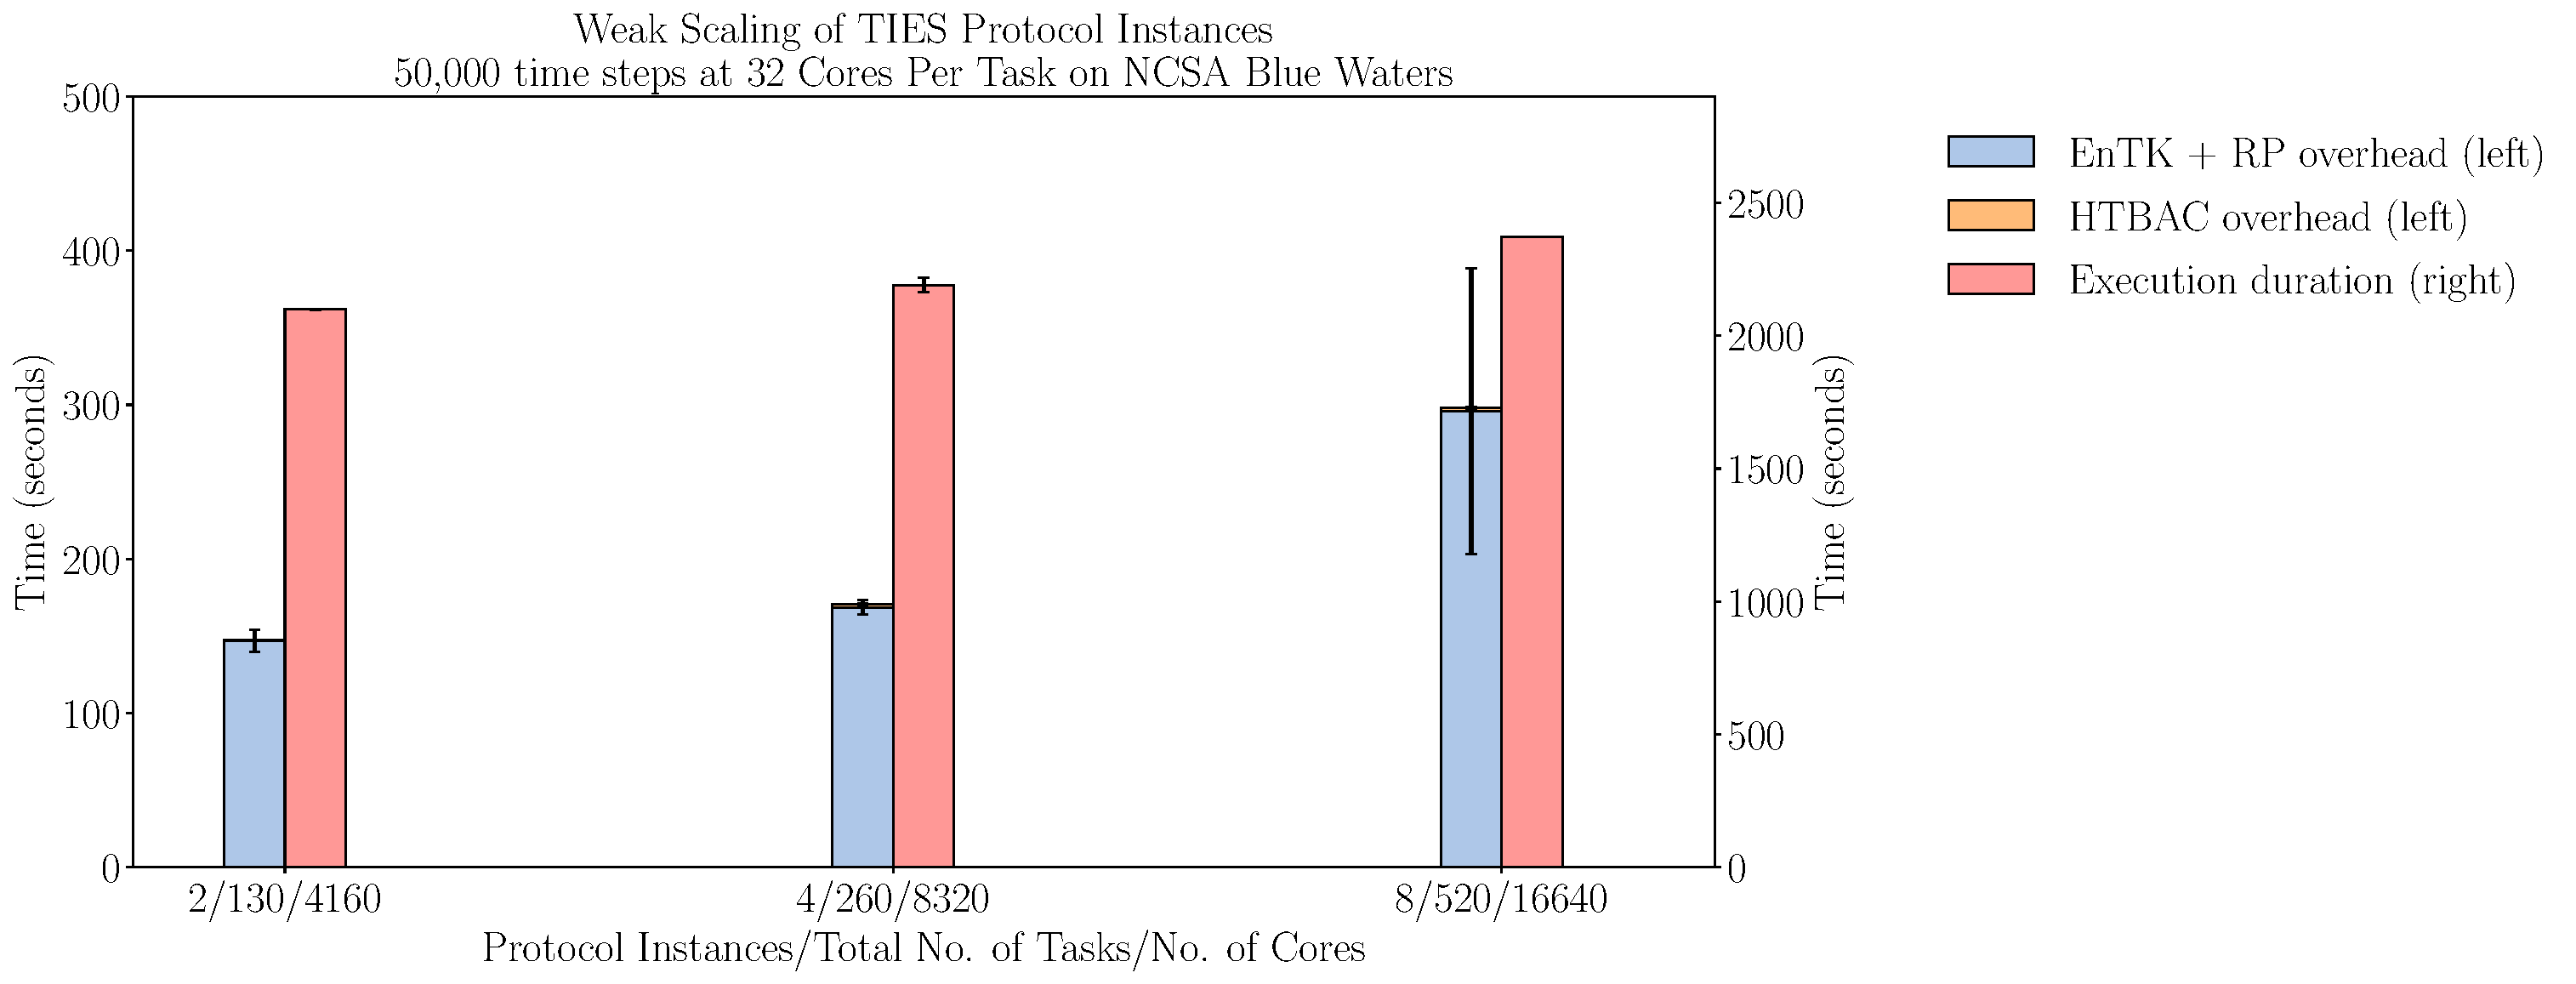
\includegraphics[width=\columnwidth]{weak_scaling_TIES_instances_50,000_timesteps.pdf}
  \caption{Weak scaling properties of HTBAC (right side). We investigate the
  weak scaling of HTBAC as the ratio of the number of protocol instances to
  resources is kept constant. (Left) Overheads of HTBAC, and runtime overhead (EnTK/RP) for
  experimental configurations investigating the weak scaling of TIES. We ran two trials for each protocol instance configuration.}
\label{fig:weak_scaling}
\end{figure}


The HTBAC overhead accounts for approximately 0.1\% of \(TTX\). The remaining
overheads, mainly EnTK and RP, depend on the number of tasks that need to be
translated in-memory from a Python object to a compute unit (CU) description.
As such, it is expected to grow proportionally to the number of tasks. EnTK
submits CU descriptions to a MongoDB used by RP, and the RP pilot pulls these
descriptions from the same database. This pull operation occurs over a wide
area networks, which introduces varying amounts of latency. In addition, each
Stage constructed by EnTK maintains sequential barriers. As such, RP remains
dormant until completion of the current Stage before staging the next State.
The impact of the barrier increases with number of CUs as seen in the 16
protocol instances data point in \ref{fig:weak_scaling}.  Together, these two
factors introduce delays in the scheduling of the CUs and results in higher
overheads. Each additional protocol instance contributes to roughly 55
additional seconds in \(TTX\).


% \(TTX\) measures the execution duration across all task, including file staging, MD kernel execution,
%  and post-executables.





%We previously demonstrated weak scaling of the ESMACS protocol in [ref SC] where we showed that a single ESMACS instance could run up to 128 concurrent pipelines.
%\jhanote{1 sentence about how pipelines in ESMACS were simpler than TIES? else the
%reader will say: you did 128 pipelines already... why should I be impressed by a
%small number of pipelines. Important to highlight that the scalability is over
%PROTOCOL INSTANCES and not pipeline instances.} \jdnote{added blurb in
%design \& implementation, removed it from here}

%\subsection{Weak/Strong Scaling Performance Results}

% Therefore our previous ESMACS experiments~\cite{} \jhanote{fix please}
% demonstrates the scalability of ESMACS as a growth in the number of pipelines.



% The goal is to isolate and understand the impact of
% increasing the number of instances, thereby the execution workload.



%The next weak scalability experiment replicates the design of the first experiment using a combination of TIES and ESMACS instances. The comparison of experiment 1 and 2 shows the ability to execute procotols with different resource requirements using one pilot.

\subsubsection {Strong Scaling Experiments}

Next we repeat the same design of the weak scalability experiments but examine
performance of strong scaling when fixing the number of pipelines and varying
the resources. The comparison between weak and strong scalability demonstrates
the overhead introduced by load balancing and scheduling tasks in multiple
generations.

(Add in additional points on strong scaling if they come in)

% HTBAC enables concurrent execution of multiple protocol instances.
% With each new protocol instance generated for an
% application, the HTBAC overhead grows to match the additional
% requirement of generating and coordinating protocols. In order
% to understand the contribution of the various events in HTBAC,
% termed as HTBAC overhead, to the total time to run, we construct the following metrics:

% \(Time-to-run = T(overhead\textsubscript{HTBAC} +
% T(overhead\textsubscript{entk}) +
% T(overhead\textsubscript{rp}) + T(execution)\). We define \(T(execution)\) as \(TTX = TTC - T_q\) where \(TTC\) is
% time-to-completion and \(T_q\) is time spent queuing on the HPC machine.

% \jhanote{We should discuss the above. It is difficult to follow..}

% The remaining overheads, mainly EnTK and RP, depend on the number of tasks
% that need to be translated in-memory from a Python object to a compute unit
% (CU) description. As such, it is expected to grow proportionally to the number
% of tasks. EnTK submits CU descriptions to a MongoDB used by RP, and the RP
% pilot pulls these descriptions from the same database. This pull operation
% occurs over a wide area networks, which introduces varying amounts of latency.

% \(TTX\) measures the execution duration across all task, which includes pre-
% executables, the main MD kernel execution, and post-executables.


\subsection{Validation Experiment Results}

To validate the fact that the HTBAC implementation of TIES we 
repeated calculations previously run by Wan \textit{et al.}
\cite{Wan2017brd4}. We selected a subset of the protein ligand systems that
were the subject of that study: they are the transforms between ligand 3 and ligands 1, 4,
and 7. We then performed a full simulation on all 3 systems and calculated the
relative binding affinities (see Table~\ref{tab:exp2}) using HTBAC.

The results show that all three $\Delta \Delta$G values are within error 
of the original study, reinforcing the fact that HTBAC has indeed correctly
implemented the complex workflow of TIES.

\begin{table}
  \centering
  \begin{tabular}{l@{\hskip 1in}r@{\hskip 0.2in}r@{\hskip 0.2in}r}
    \toprule
    System & HTBAC & Wan et. al & Experiment \\
    \midrule
    BRD4 \textbf{3 to 1} & \num{0.39 +- 0.10} &   \num{0.41 +- 0.04} &  \num{0.3 +- 0.09} \\
    BRD4 \textbf{3 to 4} & \num{0.02 +- 0.12} &   \num{0.01 +- 0.06} &  \num{0.0 +- 0.13} \\
    BRD4 \textbf{3 to 7} & \num{-0.88 +- 0.17} &  \num{-0.90 +- 0.08} & \num{-1.3 +- 0.11} \\
    \bottomrule
  \end{tabular}

  \caption{Comparison of the calculated binding free energies using HTBAC, from
  the original study by Wan \textit{et. al} and experimental data. The two theoretical
  studies used the same protcol in principle. This experiment proved that HTBAC
  has indeed implemented TIES correctly, as the calculated values are either
  the same or within error bar of the original study. All values are in
  \textbf{kcal mol\textsuperscript{-1}}.}
  \label{tab:exp2}


\end{table}

%------------------------------------------------------------------------------

\subsection{Adaptive Quadrature Experiments Results}

The impact of adaptivity is clearly seen when $\partial U/\partial\lambda$ is plotted through each iteration. 
Figure~\ref{fig:adapt} shows
how the value of $\Delta$G for one of the test systems improves as the
algorithm places more lambda windows. 

%It is imporant to note, that the new
%points are decided {\it a priori} for reasons discussed above but this is
%opaque to the algorithm. 
This is a proof that we have the adaptive capabilities
and which pave the way for more advanced biosimulation algorithms.

\begin{figure}
\begin{tikzpicture}
\begin{axis}[
  xlabel=$\lambda$,
  ylabel=$\frac{dU}{d\lambda}$,
  xmin=0,
  xmax=1,
  legend pos=outer north east,
  grid=both,
  ]
  \addplot+[name path=alch_1, mark size=1pt, mark=*, color=blue] table [x=lambda, y=p1v]{alch_1.csv};
  \addlegendentry{Iteration 1: inital lambda spacing};

  \addplot+[name path=alch_2, mark size=1pt, mark=*, color=red] table [x=lambda, y=p1v]{alch_2.csv};
  \addlegendentry{Iteration 2: Increasing number of lambda values};

  \addplot+[name path=alch_3, mark size=1pt, mark=*, color=brown] table [x=lambda, y=p1v]{alch_3.csv};
  \addlegendentry{Iteration 3: Optimial number of lambda values found};

  \addplot+[name path=alch_4, mark size=1pt, mark=*, color=black] table [x=lambda, y=p1v]{alch_4.csv};
  \addlegendentry{Iteration 4: Refining function values at optimial mesh};

  \addplot[name path=line, draw=none] {0};

  \addplot fill between[
    of = alch_1 and line,
    split,
    every even segment/.style = {pattern color=blue!50, pattern=vertical lines},
    every odd segment/.style = {pattern color=blue!50, pattern=vertical lines},
    soft clip={domain=0:1},
  ];

  \addplot fill between[
    of = alch_2 and line,
    split,
    every even segment/.style = {pattern color=red!50, pattern=horizontal lines},
    every odd segment/.style = {pattern color=red!50, pattern=horizontal lines},
    soft clip={domain=0:1},
  ];

  \addplot fill between[
    of = alch_3 and line,
    split,
    every even segment/.style = {pattern color=brown!50, pattern=north east lines},
    every odd segment/.style = {pattern color=brown!50, pattern=north east lines},
    soft clip={domain=0:1},
  ];

\end{axis}
\end{tikzpicture}
\caption{The adaptive algorithm reevaluates the efficiency of the lambda window
mesh after every \SI{1}{\nano\second} and makes a decision whether to place
more lambda windows inside certain ranges.}
\label{fig:adapt}
\end{figure}
